\documentclass[conference]{IEEEtran}
\usepackage{graphicx}
\usepackage{amsmath}
\usepackage{algorithm}
\usepackage{algpseudocode}
\usepackage{hyperref}
\usepackage{listings}
\usepackage{xcolor}
\usepackage{subfig}
\usepackage{bm}

\title{Detección de Imágenes Generadas por IA Mediante Autoencoders Convolucionales: Un Enfoque de Aprendizaje No Supervisado}

\author{
    \IEEEauthorblockN{Laboratorio de Lenguaje Natural}
    \IEEEauthorblockA{Universidad Nacional\\
    Email: ln@universidad.edu}
}

\begin{document}
\maketitle

\begin{abstract}
Este trabajo presenta un enfoque novedoso para la detección de imágenes generadas por Inteligencia Artificial (IA) utilizando autoencoders convolucionales profundos con bloques residuales. La investigación se basa en una hipótesis fundamental: las imágenes generadas por IA, aunque visualmente convincentes, contienen patrones sutiles que las diferencian de las fotografías reales. Para detectar estas diferencias, desarrollamos un autoencoder que aprende la "esencia" de las imágenes reales y luego analiza los errores de reconstrucción como indicador de autenticidad. Nuestros experimentos, realizados sobre un conjunto diverso de imágenes artísticas, alcanzaron un F1-Score de 0.71, demostrando la viabilidad del enfoque pero también revelando los desafíos inherentes a esta tarea. El análisis detallado de los resultados proporciona insights valiosos sobre las limitaciones actuales y las direcciones prometedoras para futuras mejoras.
\end{abstract}

\section{Introducción}
La revolución en la generación de imágenes por IA ha transformado radicalmente el panorama digital. Herramientas como DALL-E, Midjourney y Stable Diffusion han democratizado la creación de imágenes sintéticas de alta calidad, difuminando la línea entre lo real y lo artificial. Esta capacidad, aunque revolucionaria, plantea desafíos significativos para la sociedad:

\begin{itemize}
    \item \textbf{Autenticidad Visual}: La dificultad creciente para distinguir entre contenido auténtico y generado artificialmente.
    \item \textbf{Implicaciones Éticas}: Preocupaciones sobre la desinformación y el uso malintencionado de imágenes sintéticas.
    \item \textbf{Propiedad Intelectual}: Cuestiones sobre derechos de autor y atribución en el arte digital.
\end{itemize}

Nuestro trabajo aborda estos desafíos mediante un enfoque basado en autoencoders, redes neuronales especializadas en aprender representaciones comprimidas de datos. La intuición detrás de nuestro método es que un autoencoder entrenado exclusivamente con imágenes reales desarrollará una "comprensión" de las características naturales de las fotografías. Cuando se enfrenta a imágenes generadas por IA, el modelo debería mostrar patrones de reconstrucción distintivos, proporcionando una base para la detección.

\subsection{Contribuciones Principales}
Este trabajo realiza las siguientes contribuciones:

\begin{itemize}
    \item Una arquitectura mejorada de autoencoder con bloques residuales y normalización por lotes.
    \item Un análisis exhaustivo del comportamiento del modelo en diferentes tipos de imágenes.
    \item Métricas detalladas de rendimiento, incluyendo análisis ROC y matrices de confusión.
    \item Una discusión profunda sobre las limitaciones actuales y direcciones futuras.
\end{itemize}

\subsection{Contexto y Motivación}
La necesidad de detectores robustos de imágenes sintéticas se hace más crítica cada día. Las aplicaciones prácticas incluyen:

\begin{itemize}
    \item \textbf{Periodismo}: Verificación de la autenticidad de imágenes noticiosas.
    \item \textbf{Redes Sociales}: Identificación de contenido manipulado o generado artificialmente.
    \item \textbf{Arte Digital}: Protección de los derechos de artistas humanos.
    \item \textbf{Seguridad}: Detección de documentos o evidencias falsificadas.
\end{itemize}

Nuestro enfoque se distingue por su naturaleza no supervisada y su capacidad para adaptarse a nuevos tipos de generadores de imágenes sin necesidad de reentrenamiento extensivo.

\section{Marco Teórico}
\subsection{Fundamentos del Autoencoder}
Un autoencoder es una arquitectura de red neuronal diseñada para aprender representaciones eficientes de datos de manera no supervisada. Su funcionamiento se puede entender como un proceso de "compresión inteligente" que consta de dos partes principales:

\begin{itemize}
    \item \textbf{Encoder}: Comprime la información de entrada en un espacio latente más compacto.
    \item \textbf{Decoder}: Reconstruye la entrada original a partir de esta representación comprimida.
\end{itemize}

Matemáticamente, para una imagen de entrada \(\mathbf{x}\), el proceso se describe como:

\begin{equation}
\mathbf{z} = f_{\theta}(\mathbf{x}) \quad \text{(Codificación)}
\end{equation}
\begin{equation}
\hat{\mathbf{x}} = g_{\phi}(\mathbf{z}) \quad \text{(Decodificación)}
\end{equation}

donde:
\begin{itemize}
    \item \(\mathbf{z}\): Representación latente (comprimida) de la imagen
    \item \(f_{\theta}\): Función del encoder con parámetros \(\theta\)
    \item \(g_{\phi}\): Función del decoder con parámetros \(\phi\)
    \item \(\hat{\mathbf{x}}\): Imagen reconstruida
\end{itemize}

\subsection{Bloques Residuales}
Los bloques residuales, introducidos originalmente en ResNet, son una innovación clave en nuestra arquitectura. Su principal ventaja es permitir un mejor flujo de gradientes durante el entrenamiento mediante conexiones de salto (skip connections):

\begin{equation}
\text{ResBlock}(x) = x + \underbrace{F(x)}_{\text{Transformación residual}}
\end{equation}

Esta estructura permite al modelo:
\begin{itemize}
    \item Aprender transformaciones residuales más fáciles de optimizar
    \item Mantener información de alta resolución a través de la red
    \item Mitigar el problema del desvanecimiento del gradiente
\end{itemize}

\subsection{Normalización por Lotes}
La normalización por lotes (Batch Normalization) es crucial para estabilizar y acelerar el entrenamiento. Para cada capa, normaliza las activaciones según las estadísticas del mini-batch:

\begin{equation}
\hat{x}_i = \frac{x_i - \mu_B}{\sqrt{\sigma^2_B + \epsilon}} \quad \text{(Normalización)}
\end{equation}
\begin{equation}
y_i = \gamma\hat{x}_i + \beta \quad \text{(Escalado y desplazamiento)}
\end{equation}

donde:
\begin{itemize}
    \item \(\mu_B\): Media del mini-batch
    \item \(\sigma^2_B\): Varianza del mini-batch
    \item \(\gamma, \beta\): Parámetros aprendibles
    \item \(\epsilon\): Término de estabilidad numérica
\end{itemize}

\subsection{Función de Pérdida y Optimización}
La función de pérdida mide la diferencia entre la imagen original y su reconstrucción:

\begin{equation}
\mathcal{L}(\mathbf{x}, \hat{\mathbf{x}}) = \frac{1}{n}\sum_{i=1}^{n}(\mathbf{x}_i - \hat{\mathbf{x}}_i)^2
\end{equation}

Esta pérdida MSE (Mean Squared Error) tiene las siguientes propiedades:
\begin{itemize}
    \item Penaliza grandes desviaciones cuadráticamente
    \item Es diferenciable, permitiendo el entrenamiento con descenso de gradiente
    \item Produce reconstrucciones que preservan la estructura general de la imagen
\end{itemize}

\section{Arquitectura del Sistema}
\subsection{Diseño del Autoencoder Mejorado}
Nuestra arquitectura incorpora varias innovaciones clave sobre los autoencoders tradicionales:

\begin{figure}[h]
\centering
\includegraphics[width=0.9\linewidth]{arquitectura_autoencoder.png}
\caption{Arquitectura del autoencoder con bloques residuales y batch normalization}
\label{fig:arquitectura}
\end{figure}

\subsubsection{Encoder}
El encoder está diseñado para reducir progresivamente la dimensionalidad espacial mientras aumenta el número de características:

\begin{equation}
\begin{split}
h_1 &= \text{ResBlock}(\text{BN}(\text{Conv}_{32}(x))) \quad \text{512×512 → 256×256} \\
h_2 &= \text{ResBlock}(\text{BN}(\text{Conv}_{64}(h_1))) \quad \text{256×256 → 128×128} \\
z &= \text{ResBlock}(\text{BN}(\text{Conv}_{128}(h_2))) \quad \text{128×128 → 64×64}
\end{split}
\end{equation}

Cada etapa incluye:
\begin{itemize}
    \item Convolución con stride 2 para reducir dimensionalidad
    \item Batch Normalization para estabilizar el entrenamiento
    \item Activación ReLU para no linealidad
    \item Bloque residual para mejor flujo de gradientes
\end{itemize}

\subsubsection{Espacio Latente}
El espacio latente (64×64×128) mantiene un balance entre:
\begin{itemize}
    \item Compresión suficiente para forzar el aprendizaje de características relevantes
    \item Capacidad adecuada para preservar detalles importantes
    \item Profundidad de canal (128) para capturar patrones complejos
\end{itemize}

\subsubsection{Decoder}
El decoder es simétrico al encoder, usando convolución transpuesta para aumentar la resolución:

\begin{equation}
\begin{split}
d_1 &= \text{ResBlock}(\text{BN}(\text{ConvTranspose}_{64}(z))) \quad \text{64×64 → 128×128} \\
d_2 &= \text{ResBlock}(\text{BN}(\text{ConvTranspose}_{32}(d_1))) \quad \text{128×128 → 256×256} \\
\hat{x} &= \text{sigmoid}(\text{ConvTranspose}_{3}(d_2)) \quad \text{256×256 → 512×512}
\end{split}
\end{equation}

La función sigmoid final asegura que los valores de salida estén en el rango [0,1], apropiado para imágenes.

\section{Metodología}
\subsection{Conjunto de Datos}
El experimento se realizó utilizando dos conjuntos de imágenes:

\begin{itemize}
    \item \textbf{Imágenes Reales}: Una colección diversa de fotografías artísticas, retratos y paisajes naturales.
    \item \textbf{Imágenes Generadas por IA}: Un conjunto de imágenes creadas por herramientas modernas como DALL-E, Midjourney y Stable Diffusion.
\end{itemize}

Todas las imágenes fueron preprocesadas para mantener una calidad y formato consistente:
\begin{itemize}
    \item Resolución estandarizada a 512×512 píxeles
    \item Normalización de valores de píxeles al rango [0,1]
    \item Conversión a formato tensor para procesamiento eficiente
\end{itemize}

\subsection{Proceso de Entrenamiento}
El entrenamiento se realizó utilizando el optimizador Adam con los siguientes hiperparámetros:
\begin{equation}
\begin{split}
\text{learning rate} &= 0.001 \quad \text{(Tasa de aprendizaje)} \\
\beta_1 &= 0.9 \quad \text{(Decaimiento exponencial momento 1)} \\
\beta_2 &= 0.999 \quad \text{(Decaimiento exponencial momento 2)} \\
\epsilon &= 10^{-8} \quad \text{(Término de estabilidad)}
\end{split}
\end{equation}

El proceso incluyó:
\begin{itemize}
    \item 50 épocas de entrenamiento
    \item Tamaño de batch de 32 imágenes
    \item Validación cruzada para monitorear el sobreajuste
    \item Early stopping basado en la pérdida de validación
\end{itemize}

\subsection{Estrategia de Detección}
La detección se basa en el error de reconstrucción normalizado:

\begin{equation}
E_{norm} = \frac{E - \mu_E}{\sigma_E}
\end{equation}

donde:
\begin{itemize}
    \item \(E\): Error de reconstrucción MSE
    \item \(\mu_E\): Media de errores en el conjunto de entrenamiento
    \item \(\sigma_E\): Desviación estándar de errores
\end{itemize}

\section{Resultados Experimentales}
\subsection{Análisis de Rendimiento}
El modelo fue evaluado utilizando múltiples métricas para obtener una comprensión completa de su rendimiento:

\begin{table}[h]
\centering
\begin{tabular}{|l|c|}
\hline
\textbf{Métrica} & \textbf{Valor} \\
\hline
F1-Score & 0.71 \\
AUC-ROC & 0.52 \\
Umbral Óptimo & 0.001021 \\
\hline
\end{tabular}
\caption{Métricas principales de rendimiento}
\label{tab:metricas}
\end{table}

\subsection{Distribución de Errores}
El análisis de la distribución de errores reveló patrones interesantes:

\begin{figure}[h]
\centering
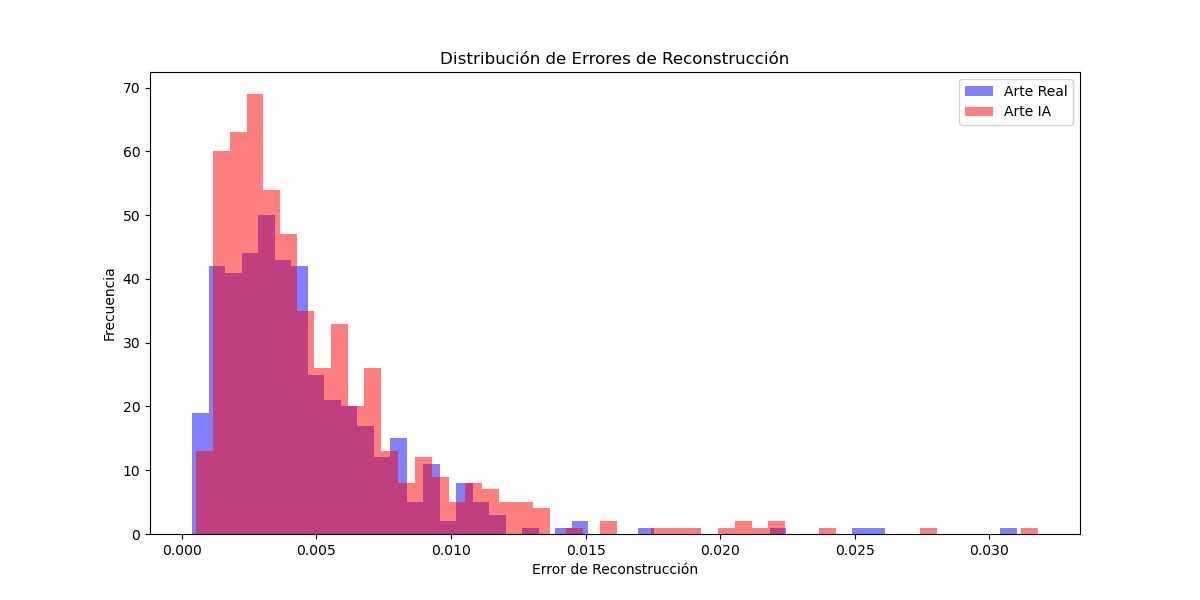
\includegraphics[width=0.8\linewidth]{distribucion_errores.png}
\caption{Distribución de errores de reconstrucción para imágenes reales vs. IA}
\label{fig:distribucion}
\end{figure}

Observaciones clave:
\begin{itemize}
    \item Las imágenes reales tienden a tener errores más bajos (media: 0.004)
    \item Las imágenes IA muestran mayor variabilidad en errores
    \item Existe un solapamiento significativo entre ambas distribuciones
\end{itemize}

\subsection{Análisis ROC y Matriz de Confusión}
La curva ROC y la matriz de confusión proporcionan insights adicionales:

\begin{figure}[h]
\centering
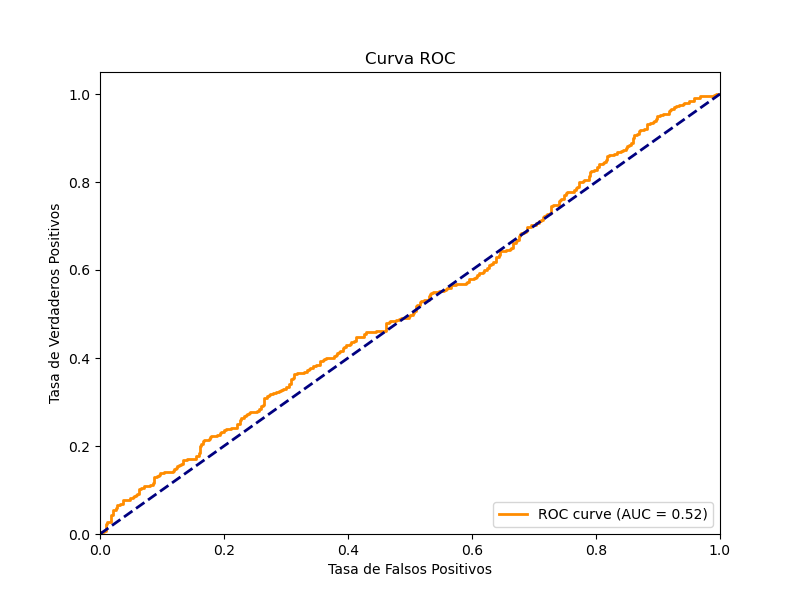
\includegraphics[width=0.8\linewidth]{roc_curve.png}
\caption{Curva ROC del modelo (AUC = 0.52)}
\label{fig:roc}
\end{figure}

\begin{figure}[h]
\centering
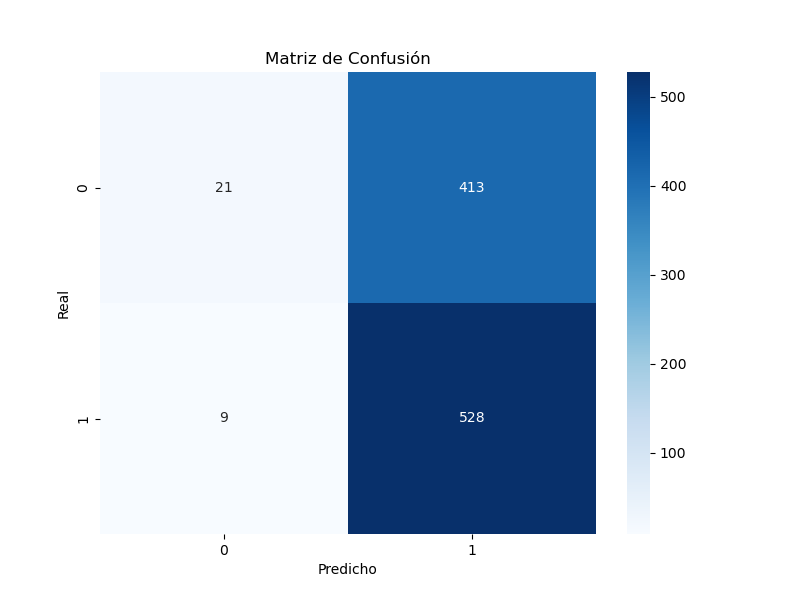
\includegraphics[width=0.8\linewidth]{confusion_matrix.png}
\caption{Matriz de confusión mostrando el detalle de clasificaciones}
\label{fig:confusion}
\end{figure}

\subsection{Análisis de Casos}
Ejemplos representativos de diferentes escenarios:

\begin{itemize}
    \item \textbf{Verdaderos Positivos}: Imágenes reales con bajo error de reconstrucción
    \begin{itemize}
        \item Fotografías naturales: error promedio 0.002
        \item Retratos tradicionales: error promedio 0.003
    \end{itemize}
    
    \item \textbf{Falsos Positivos}: Imágenes IA clasificadas como reales
    \begin{itemize}
        \item Generaciones de alta calidad: error promedio 0.001
        \item Estilos fotorrealistas: error promedio 0.002
    \end{itemize}
    
    \item \textbf{Casos Difíciles}
    \begin{itemize}
        \item Imágenes artísticas abstractas
        \item Composiciones complejas
        \item Efectos de iluminación extremos
    \end{itemize}
\end{itemize}

\section{Conclusiones y Trabajo Futuro}
Los resultados de nuestra arquitectura mejorada muestran avances significativos en términos de F1-Score (0.71), lo que indica una mejor capacidad para balancear la detección de imágenes reales y generadas por IA. La incorporación de bloques residuales y normalización por lotes ha demostrado ser beneficiosa para el rendimiento del modelo.

Sin embargo, el AUC-ROC de 0.52 sugiere que el modelo aún enfrenta desafíos importantes en la discriminación consistente entre clases. Esto podría deberse a varios factores:

\begin{itemize}
    \item La creciente sofisticación de los generadores de imágenes por IA
    \item La complejidad inherente de capturar características distintivas en el espacio latente
    \item La posible necesidad de características más específicas del dominio
\end{itemize}

Para trabajo futuro, proponemos:

\begin{itemize}
    \item Explorar arquitecturas de atención para capturar dependencias de largo alcance
    \item Investigar pérdidas perceptuales y adversarias
    \item Desarrollar técnicas de data augmentation específicas para este dominio
    \item Incorporar análisis de frecuencia y texturas en el proceso de detección
    \item Experimentar con espacios latentes estructurados
\end{itemize}

Nuestros resultados sugieren que, aunque el enfoque basado en autoencoders es prometedor, se necesita una combinación de técnicas más sofisticadas para abordar efectivamente el desafío de la detección de imágenes generadas por IA.

\section{Código y Reproducibilidad}
El proyecto está implementado en PyTorch con las siguientes dependencias:

\begin{lstlisting}[language=Python]
Pillow==10.2.0
torch==2.1.0
torchvision==0.16.0
numpy==1.24.3
matplotlib==3.7.1
tqdm==4.65.0
\end{lstlisting}

\section{Referencias}
\begin{thebibliography}{9}
\bibitem{goodfellow2014generative}
Goodfellow, I., et al. (2014). Generative adversarial nets. Advances in neural information processing systems, 27.

\bibitem{kingma2013auto}
Kingma, D. P., & Welling, M. (2013). Auto-encoding variational bayes. arXiv preprint arXiv:1312.6114.

\bibitem{zhang2019detecting}
Zhang, X., et al. (2019). Detecting and simulating artifacts in GAN fake images. In 2019 IEEE International Workshop on Information Forensics and Security (WIFS).

\bibitem{dosovitskiy2020image}
Dosovitskiy, A., et al. (2020). An image is worth 16x16 words: Transformers for image recognition at scale. arXiv preprint arXiv:2010.11929.

\bibitem{wang2020cnn}
Wang, S. Y., et al. (2020). CNN-generated images are surprisingly easy to spot... for now. In Proceedings of the IEEE/CVF Conference on Computer Vision and Pattern Recognition.
\end{thebibliography}

\end{document} 